\section{Estado de arte}


%%%%%%%%%%%%%%%%%%%%%%%%%%%%%%%%%%%%%%%%%%%%%%%%%%%%%%%%%%%%%%%%%%%%%%%%%%%%%%%%%%%%%%%%
\begin{frame}
\frametitle{\citetitle{Allen1976BodyLI}}
\begin{figure}[!ht]
    \centering
    \caption{Linguagem corporal na sala do médico (Fonte: \textcite{Allen1976BodyLI}).}
    \begin{minipage}[t]{0.24\textwidth}
      \centering
      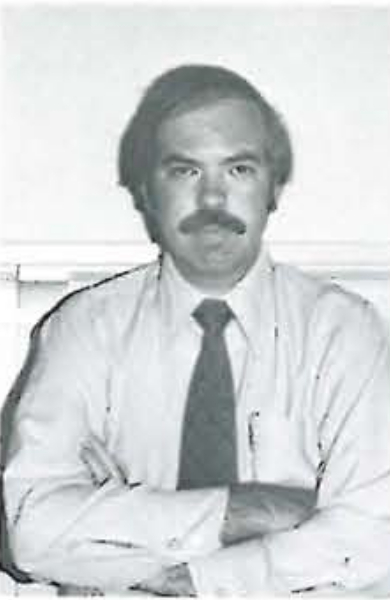
\includegraphics[width=0.8\textwidth]{images/dentista1.jpg}
      \subcaption{Braços cruzados sobre o peito. Indica frialdade e indiferença.\label{fig:Allen1976BodyLI:1:A}}
    \end{minipage}
    \hfill
    \begin{minipage}[t]{0.24\textwidth}
      \centering
      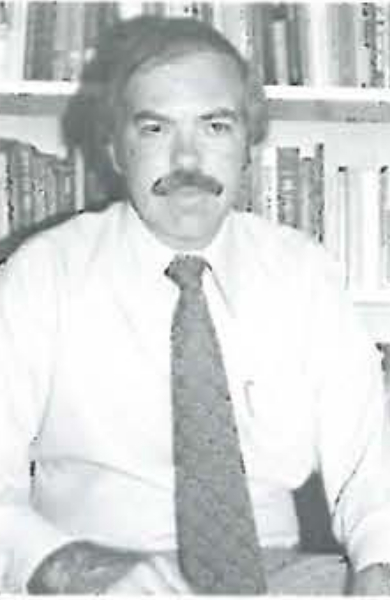
\includegraphics[width=0.8\textwidth]{images/dentista2.jpg}
      \subcaption{Ligeiramente para a frente, costas curvadas e braços relaxados.
      Indica uma abertura à comunicação.\label{fig:Allen1976BodyLI:1:B}}
    \end{minipage}
    \hfill
    \begin{minipage}[t]{0.24\textwidth}
      \centering
      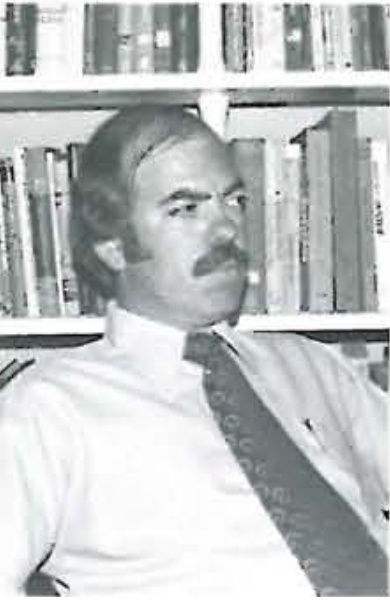
\includegraphics[width=0.8\textwidth]{images/dentista3.jpg}
      \subcaption{Reclinado para o mais longe possível, 
      cara e olhos apontando para longe do orador. Má escuta.\label{fig:Allen1976BodyLI:1:C}}
    \end{minipage}
    \hfill
    \begin{minipage}[t]{0.24\textwidth}
      \centering
      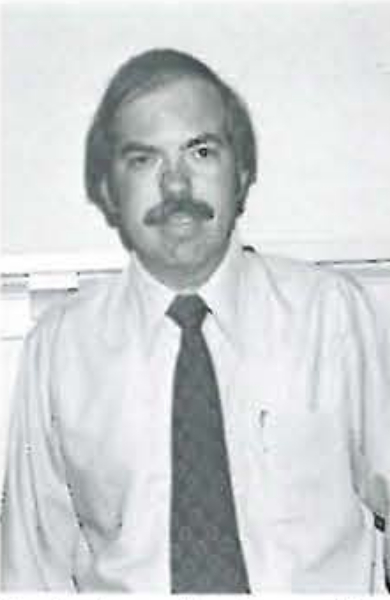
\includegraphics[width=0.8\textwidth]{images/dentista4.jpg}
      \subcaption{Leve sorriso, os braços pendurados nas laterais.
      Esta é a melhor saudação para o interlocutor.\label{fig:Allen1976BodyLI:1:D}}
    \end{minipage}
    \label{fig:Allen1976BodyLI:1}
  \end{figure}
\end{frame}

%%%%%%%%%%%%%%%%%%%%%%%%%%%%%%%%%%%%%%%%%%%%%%%%%%%%%%%%%%%%%%%%%%%%%%%%%%%%%%%%%%%%%%%%
\begin{frame}
    \frametitle{\citetitle{Edmondstone1995CardiacCP}}
    Pacientes na unid. coronariana: 77\% isquemia cardíaca.
    \begin{figure}[!ht]
        \centering
        \caption{Linguagem corporal de um paciente cardíaco 
        e a mensagem que carrega (Fonte: \textcite{Edmondstone1995CardiacCP}).}
        \begin{minipage}[t]{0.24\textwidth}
          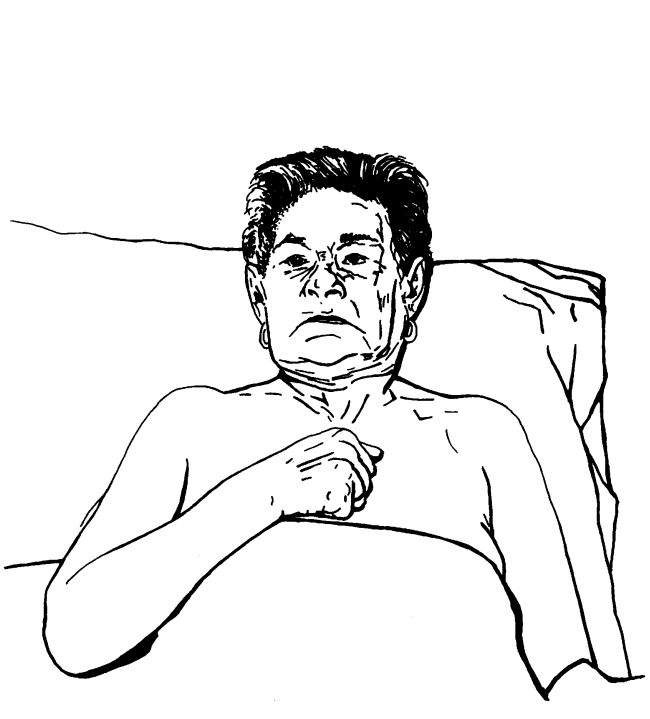
\includegraphics[width=0.95\textwidth]{images/cardiac1.jpg}
          \subcaption{Punho cerrado no meio do peito (sinal de Levine). \label{fig:Edmondstone1995CardiacCP:1}}
        \end{minipage}
        \hfill
        \begin{minipage}[t]{0.24\textwidth}
          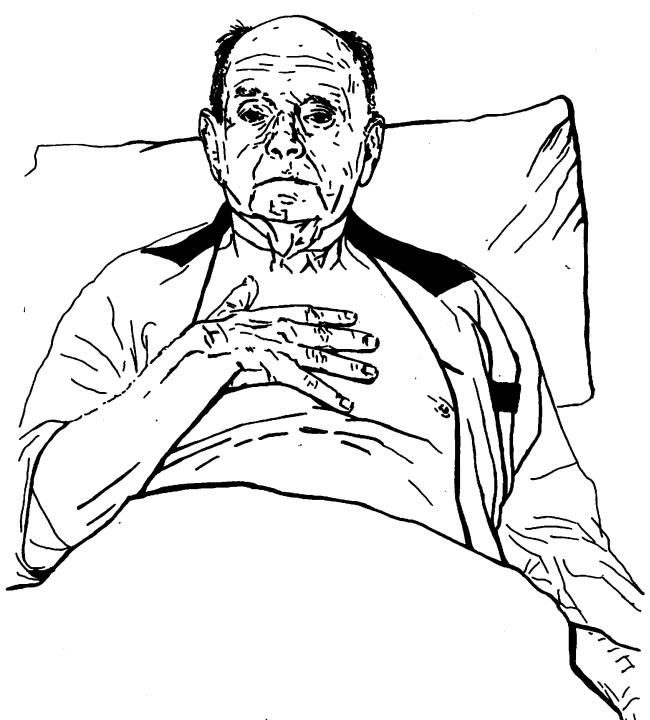
\includegraphics[width=0.95\textwidth]{images/cardiac2.jpg}
          \subcaption{Palma da mão no centro do peito. \label{fig:Edmondstone1995CardiacCP:2}}
        \end{minipage}
        \hfill
        \begin{minipage}[t]{0.24\textwidth}
          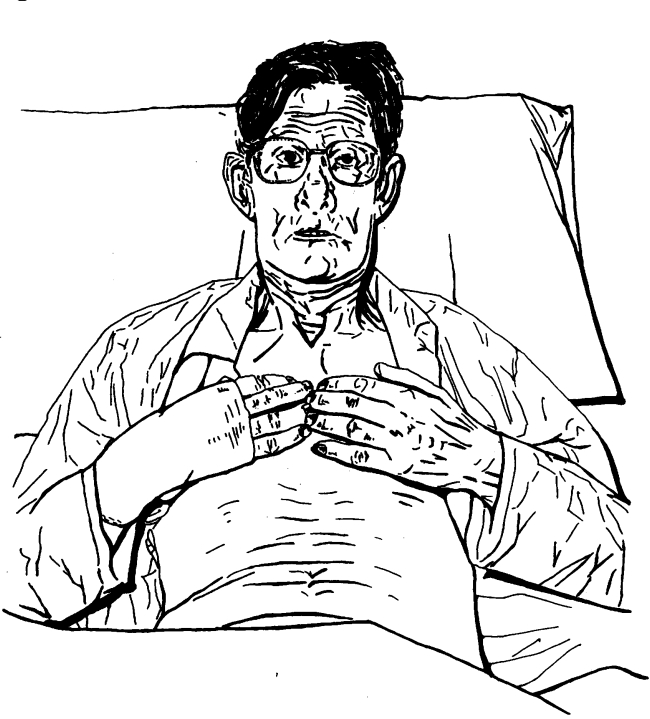
\includegraphics[width=0.95\textwidth]{images/cardiac3.jpg}
          \subcaption{Ambas as mãos colocadas no meio do peito. \label{fig:Edmondstone1995CardiacCP:3}}
        \end{minipage}
        \label{fig:Edmondstone1995CardiacCP}
      \end{figure}
    \end{frame}

%%%%%%%%%%%%%%%%%%%%%%%%%%%%%%%%%%%%%%%%%%%%%%%%%%%%%%%%%%%%%%%%%%%%%%%%%%%%%%%%%%%%%%%%
\begin{frame}
    \frametitle{\citetitle{van2007body}}
    Reconhecimento de emoções - expressões corporais (p-valor)
    \begin{figure}[!ht]
        \centering
        \caption{Uma expressão de raiva no topo (alvo) e no canto inferior direito. 
        Uma expressão triste no canto inferior esquerdo (Fonte: \textcite{van2007body}).}
          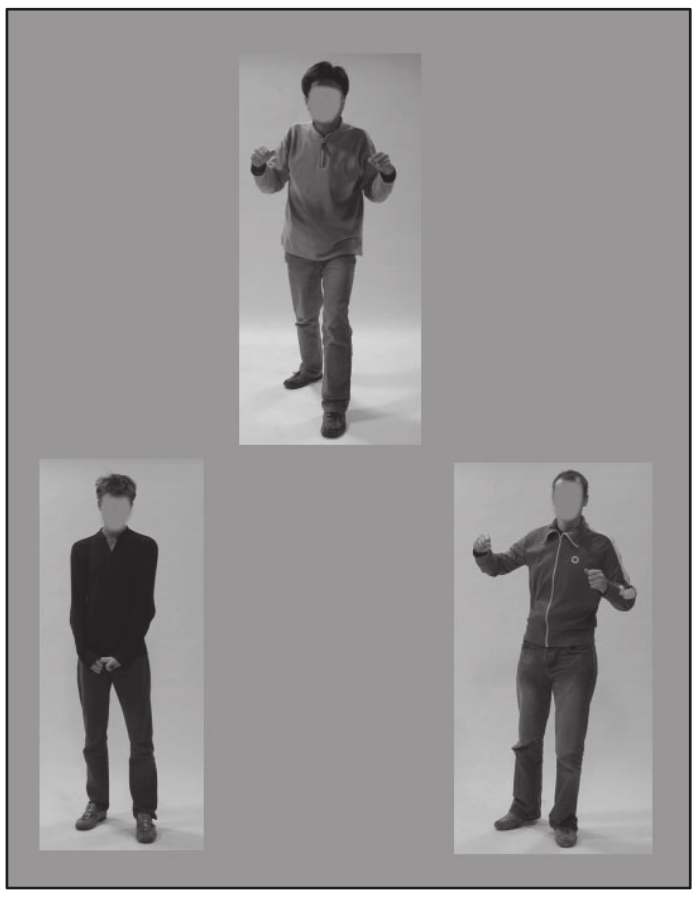
\includegraphics[width=0.27\textwidth]{images/van2007body0.png}
        \label{fig:van2007body}
    \end{figure}
\end{frame}
%%%%%%%%%%%%%%%%%%%%%%%%%%%%%%%%%%%%%%%%%%%%%%%%%%%%%%%%%%%%%%%%%%%%%%%%%%%%%%%%%%%%%%%%
\begin{frame}
    \frametitle{\citetitle{van2007body}}
    Categorizar a expressão facial - Respostas elétricas do cérebro (p-valor)
    \begin{figure}[!ht]
        \centering
        \caption{Exemplos mostrando uma expressão corporal feliz com uma face 
        transformada. 
        Esquerda: 100\% com medo; direita: 100\% feliz (Fonte: \textcite{van2007body}).}
          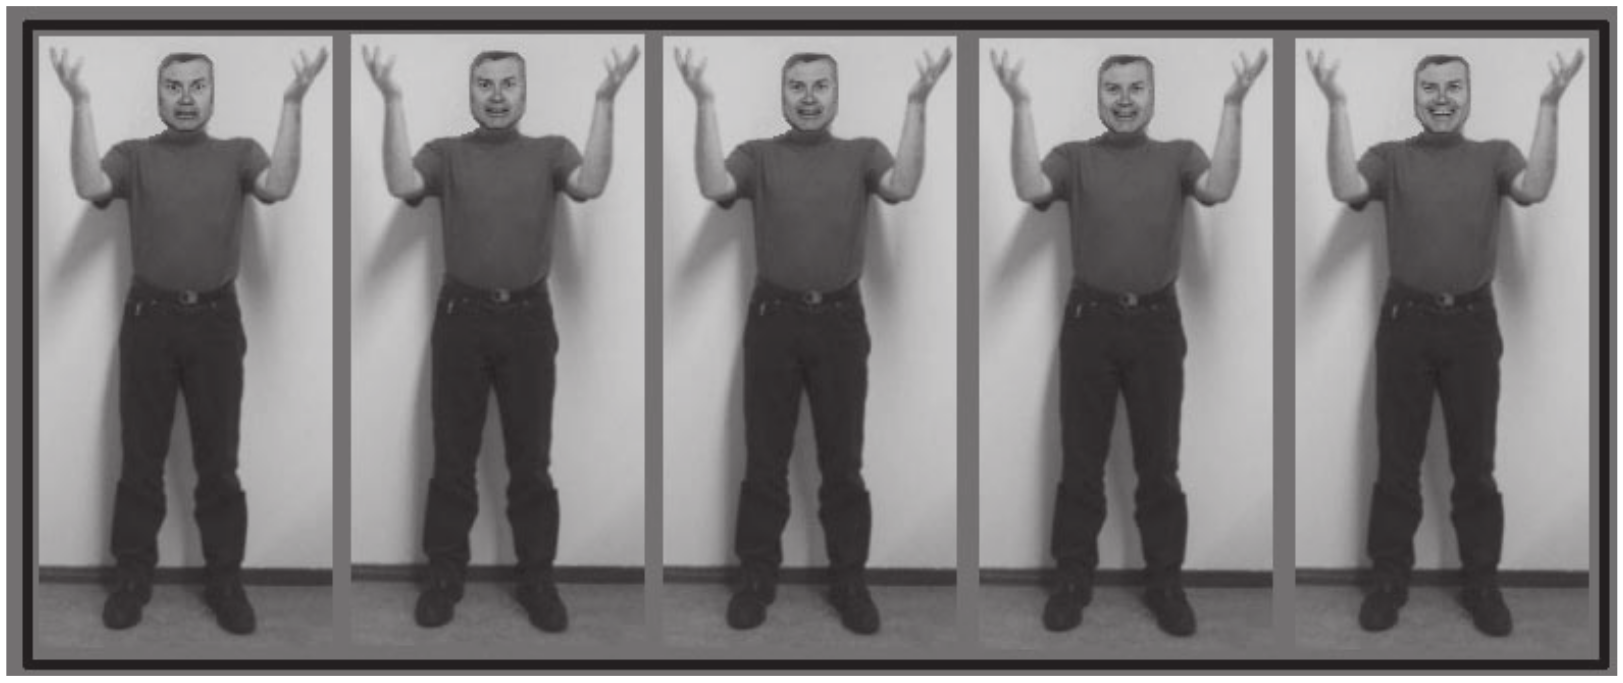
\includegraphics[width=0.85\textwidth]{images/van2007body.png}
        \label{fig:van2007body:2}
    \end{figure}
\end{frame}

%%%%%%%%%%%%%%%%%%%%%%%%%%%%%%%%%%%%%%%%%%%%%%%%%%%%%%%%%%%%%%%%%%%%%%%%%%%%%%%%%%%%%%%%
\begin{frame}
    \frametitle{\citetitle{bargshady2019joint}} 
    48 mil imagens: 200 sequencias de vídeo, 25 pessoas. 
VGGFace+RNN, o sistema obteve 75.2\% de acuracia.
    \begin{figure}[!ht]
    \centering
    \caption{Banco de dados UNBC McMaster em diferentes níveis de 
    dor e pontuação PSPI (Fonte: \textcite{bargshady2019joint}).}
      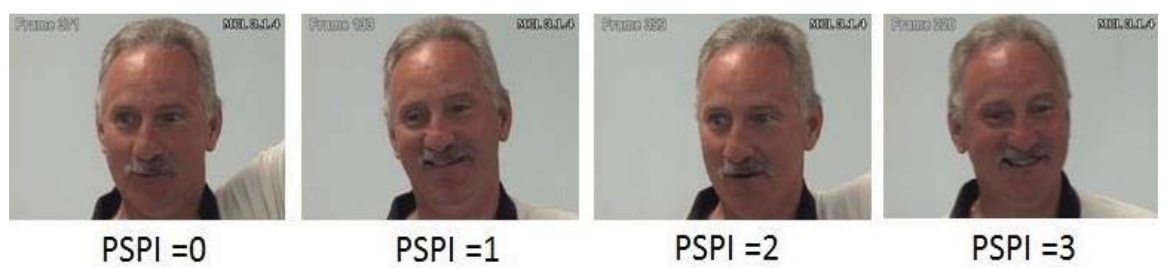
\includegraphics[width=0.9\textwidth]{images/bargshady2019joint.png}
    \label{fig:bargshady2019joint}
  \end{figure}
\end{frame}


%%%%%%%%%%%%%%%%%%%%%%%%%%%%%%%%%%%%%%%%%%%%%%%%%%%%%%%%%%%%%%%%%%%%%%%%%%%%%%%%%%%%%%%%
\begin{frame}
    \frametitle{\citetitle{chen2019real}}
3xConv2D + 2xDense. 
O sistema obteve 83\% de acuracia (49 imagens).
\begin{figure}[!ht]
    \centering
    \caption{Base de dados com imagens de pessoas no hospital (Fonte: \textcite{chen2019real}).}
    \begin{minipage}[t]{0.45\textwidth}
    \centering
      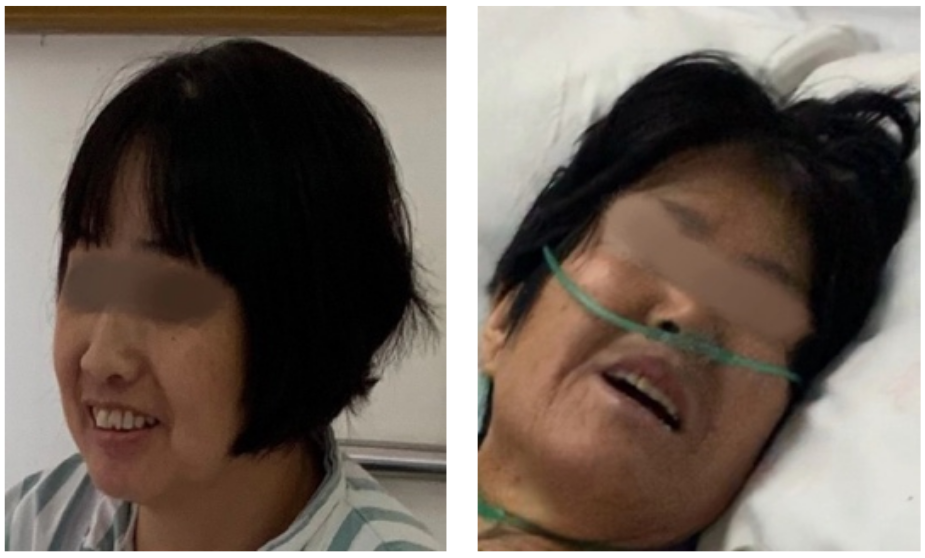
\includegraphics[width=0.95\textwidth]{images/chen2019real-a.png}
      \subcaption{Imagens de uma pessoa em estados normais (sem dor). \label{fig:chen2019real:1}}
    \end{minipage}
    \hfill
    \begin{minipage}[t]{0.45\textwidth}
    \centering
      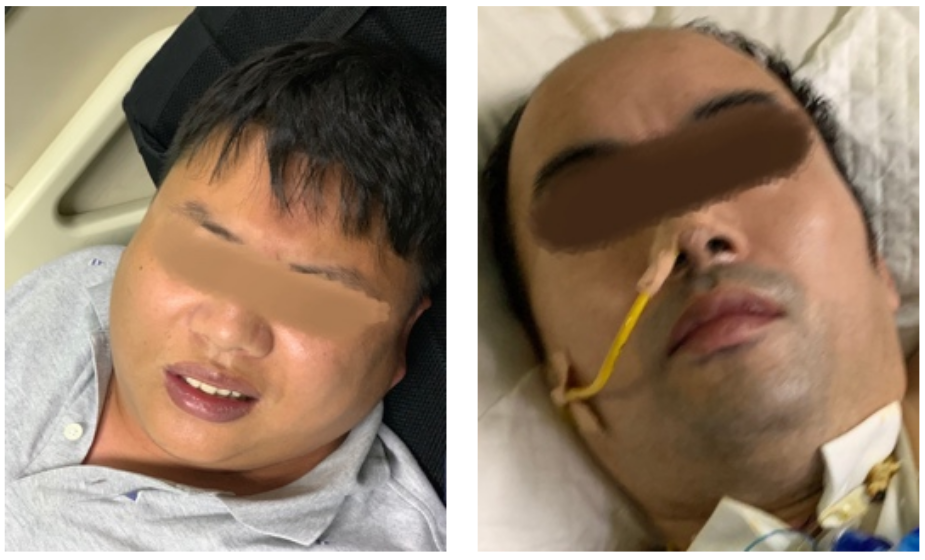
\includegraphics[width=0.95\textwidth]{images/chen2019real-b.png}
      \subcaption{Imagens de uma pessoa em estados abnormais (dor). \label{fig:chen2019real:2}}
    \end{minipage}
    \label{fig:chen2019real}
  \end{figure}
\end{frame}

%%%%%%%%%%%%%%%%%%%%%%%%%%%%%%%%%%%%%%%%%%%%%%%%%%%%%%%%%%%%%%%%%%%%%%%%%%%%%%%%%%%%%%%%
\begin{frame}
    \frametitle{\citetitle{BadrulhishamMangshor2021}}
    
O sistema obteve uma acurácia 92.5\%. (80 imagens)
\begin{figure}[!ht]
    \centering
    \caption{Expressões faciais (Fonte: \textcite{BadrulhishamMangshor2021}).}
      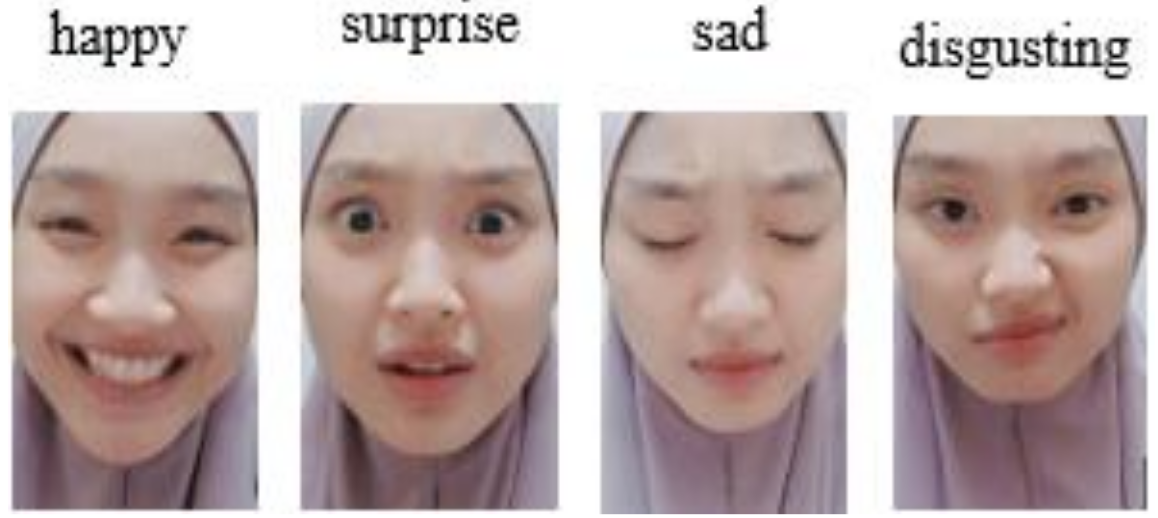
\includegraphics[width=0.7\textwidth]{images/BadrulhishamMangshor2021.png}
    \label{fig:BadrulhishamMangshor2021}
\end{figure}

\end{frame}
